\chapter{IMPLEMENTANDO LEAN EM UMA EMPRESA DE SOFTWARE}

Esse trabalho, como identificado na sessão \ref{chap1:obj}, tem como objetivo propor uma melhoria no modelo de desenvolvimento de uma empresa de \textit{software} aplicando conceitos do \textit{lean}. Assim, esse capítulo aborda o processo de desenvolvimento atual e tenta melhora-lo com alguns  dos princípios do desenvolvimento \textit{lean} de \textit{software} vistos no Capítulo \ref{cha:lean}.

\section{A EMPRESA}

Nesse capítulo é descrito o processo de desenvolvimento de uma empresa de \textit{software} do ramo de auto publicação de livros. O nome da empresa não é mencionado, mas isso não contribui de forma negativa para o trabalho proposto. A empresa possui atualmente três sistemas, os quais foram desenvolvidos utilizando-se a linguagem de programação ruby. Além da linguagem ruby, é utilizado o \textit{framework} Rails, já que os produtos são plataformas SAAS (\textit{Software as a Service}). Outras tecnologias utilizadas são: AWS (\textit{Amazon Web Services}), para armazenamento de arquivos e imagens na núvem, Postgres SQL (para banco de dados) e outras tecnologias. 

No que tange a equipe de desenvolvimento, a equipe foi composta até pouco tempo por três programadores, e hoje conta apenas com um engenhairo de \textit{software} que é responsável por atender solicitações do dono do negócio (ou \textit{Product Owner} no Scrum). Esse profissional é responsável pela parte de \textit{backend} (lógica de negócios), \textit{frontend} e suporte técnico (quando necessário). A análise técnica e estimativa também é feita por esse profissional. Um time de atendimento ao usuário (duas pessoas) também existe, o qual passa as demandas de suporte técnico (quando existem) via Zendesk (ferramenta de suporte). Alguns pontos de melhorias anteriores a esse trabalho contribuíram para a implantação do \textit{lean}, então essas melhorias também são mencionadas. A sessão seguinte mostra o processo utilizado atualmente.

\section{O PROCESSO DE SOFTWARE ATUAL}
\label{sec:processo_atual}

Para implementar o desenvolvimento \textit{lean} em uma empresa, como visto no capítulo anterior, é fundamental identificar e conhecer o processo de \textit{software} e identificar os desperdícios como visto na sessão \ref{sec:desperdicios}. Na Figura \ref{fig:processo_atual} é mostrado o fluxo básico da empresa atualmente. Tudo começa com o \textit{backlog} de produto. O \textit{backlog} de produto foi um componente tirado do Scrum (visto na sessão \ref{sec:scrum}). Atualmente utiliza-se um modelo de Scrum, mas sem algumas cerimônias como \textit{daily meeting}, já que todo o processo é feito hoje apenas por uma pessoa. O \textit{product owner} é responsável por colocar os itens e priorizar o \textit{backlog}. Através de uma reunião, os items são colocados em um \textit{backlog} de \textit{sprint}, que vão compor uma \textit{sprint} que dura de 2 até 3 semanas. Quando iniciada a \textit{sprint}, o desenvolvimento de uma funcionalidade vai seguir um modelo incremental: não necessáriamente em um ciclo a funcionalidade toda vai acabar. Cada vez que uma funcionalidade estiver pronta, pode-se enviar para o ambiente de homologação para os \textit{stakeholders} validarem e darem um \textit{feedback}. Testes efetuados por terceiros são feitos em projetos maiores (embora não estejam representados no processo). Caso a funcionalidade seja validada, ela pode ser enviada para produção. Quando todas as funcionalidades estiverem prontas, a \textit{sprint} termina.

\begin{figure}[htb!]
\begin{center}
\caption{Processo de desenvolvimento atual com desperdício identificado}
\label{fig:processo_atual}
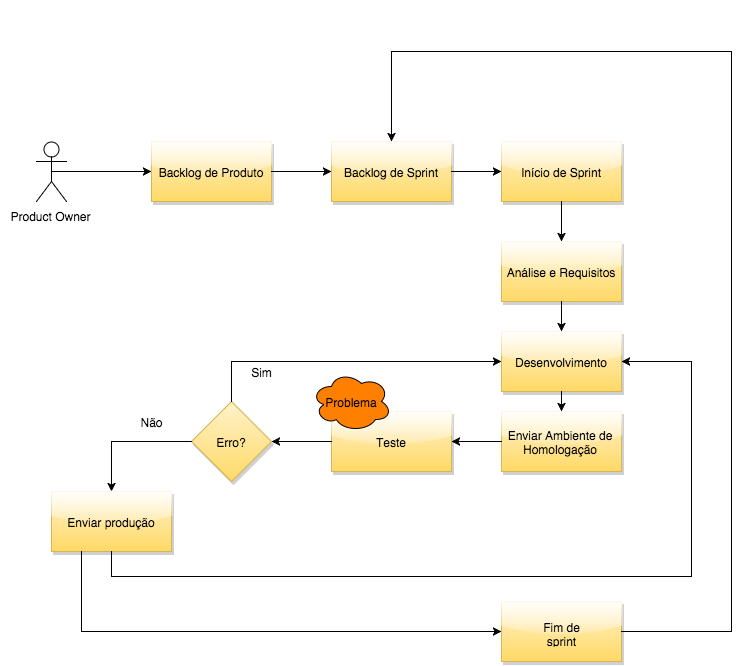
\includegraphics[width=12cm]{assets/compreender_problema} \\
\fonte{Autoria própria}
\end{center}
\end{figure}


\section{IDENTIFICANDO DESPERDÍCIOS}
\label{sec:identificando_despercio}

Um dos problemas apontados na Figura \ref{fig:processo_atual} da sessão \ref{sec:processo_atual} é apontado na nuvem identificada com a palavra ``problema''. O sistema principal da empresa, que está em foco nesse trabalho e representa mais de 80\% da renda da empresa, foi construido sem as técnicas apresentadas na sessão \ref{sec:quality} como TDD e BDD. Toda vez que uma alteração no sistema precisa ser feita, não há como prever se alguma funcionalidade existente pode ser afetada. Se o sistema fosse construído com o uso de TDD e BDD, os testes seriam rodadas em cada \textit{deploy}, e caso algum comportamento do sistema falhasse, o código teria que ser reescreito, o que evitaria de enviar novos problemas para produção. Esse tipo de problema fere claramente o princípio da eliminação de desperdício e da incorporação de qualidade. No \textit{lean}, como visto no Capítulo \ref{cha:lean}, é preciso não apenas garantir o teste depois da codificação, mas trabalhar na questão de detecção do erro. Em uma analogia com o sistema Toyota de manufatura, toda vez que houver algum problema na linha de produção, esse problema deve ser detectado e a linha de produção deve parar para que o problema ou defeito seja corrigido. Uma das maneiras de se identificar esses desperdícios é montando o fluxo da empresa em um gráfico que pode ser um diagrama de fluxo de valor como mostra a Figura \ref{fig:01} no Capítulo \ref{chap:01} ou de forma mais simples como identificado na Figura \ref{fig:processo_atual}.

\section{RESOLVENDO DESPERDÍCIO}

Como mencionado na sessão \ref{sec:identificando_despercio}, existe um problema que faz com que novos suportes e \textit{tickets} no Zendesk sejam frequentes cada vez que uma ou mais novas funcionalidades entrem no ar. Devido a complexidade do sistema, é praticamente impossível e até mesmo inviável (devido a presença de apenas uma pessoa na equipe) que se teste o sistema inteiro sempre que uma nova funcionalidade seja enviada para o ambiente de produção. Mas qual a melhor alternativa para resolver problemas de teste em sistemas legados com nenhuma cobertura de testes ? 

\begin{figure}[htb!]
\begin{center}
\caption{Tipos de testes}
\label{fig:tipo_testes}
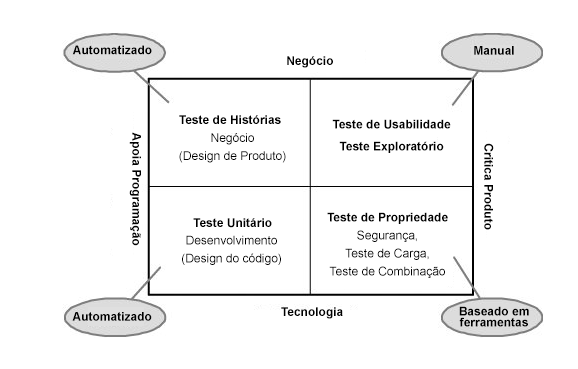
\includegraphics[width=14cm]{assets/testetab} \\
\fonte{\citeauthoronline{poppendieck:07}, \citeyear{poppendieck:07}.}
\end{center}
\end{figure}

A Figura \ref{fig:tipo_testes} mostra os tipos de testes existentes e suas finalidades. Como pode-se observar, os testes podem estar mais relacionados com questões de negócio ou tecnológicas. Ao mesmo tempo ele pode apoiar mais a programação em si ou fazer críticas ao \textit{software}. Um teste de usabilidade (relacionado ao segundo quadrante superior), por exemplo, poderia encontrar problemas relacionados a dificuldade de se encontrar alguma coisa na tela, ou a realizar alguma ação etc. Esse tipo de testes geralmente é executado por alguma pessoa, e já é realizado na empresa. Os testes de negócio e unitários foram descritos na sessão \ref{sec:quality}. Os testes de propriedade podem testar questões relacionadas a segurança do sistema, carga e combinação. Frequentemente pode-se utilizar ferramentas prontas para, por exemplo, achar vulnerabilidades conhecidas em códigos, pastas com permissões indevidas etc. Um exemplo desse tipo de ferramente de teste de propriedade é o WPSCan\footnote{O WPScan pode ser encontrado e baixado no endereço http://bit.ly/1MPrh2w.}, que procura vulnerabilidades em um sistema feito com Wordpress.

No caso do sistema da empresa em questão, é importante garantir que as novas funcionalidades sejam feitas utilizando-se do princípio do TDD e BDD, pois ele garante que o desenvolvimento seja maduro através do processo de \textit{design} do código e da refatoração, que se encaixa no \textit{seiri} (organização) no 5S do \textit{lean}. Em casos como esse, em que há pouca cobertura de teste, é preciso saber o que testar. Nesse caso, é indispensável que funcionalidades essenciais do sistema estejam coberta por testes.

Como mencionado no início do capítulo, o sistema da empresa foi implementado com o \textit{framework} Rails. Houve uma demanda do suporte de mudança no cadastro de usuários: que é uma parte crítica do sistema. Basicamente a ficha cadastral foi combinada com outra ficha de cadastro relacionada aos autores (que antes era separada). Uma das maneiras de se testar que tudo sempre vai funcionar como esperado é implementar teste de \textit{views}. Utilizando o \textit{Selenium Web Browser} com uma ferramenta chamada Capybara\footnote{O projeto Capybara pode ser encontrado no endereço http://bit.ly/1ht90TA.}, que torna a escrita de testes que utilizam-se do Selenium mais fácil, foi possível escrever testes que são codificados uma vez e que vão executar automaticamente de forma lógica. 

\begin{figure}[htb!]
\begin{center}
\caption{Teste de \textit{View}}
\label{fig:teste_view}
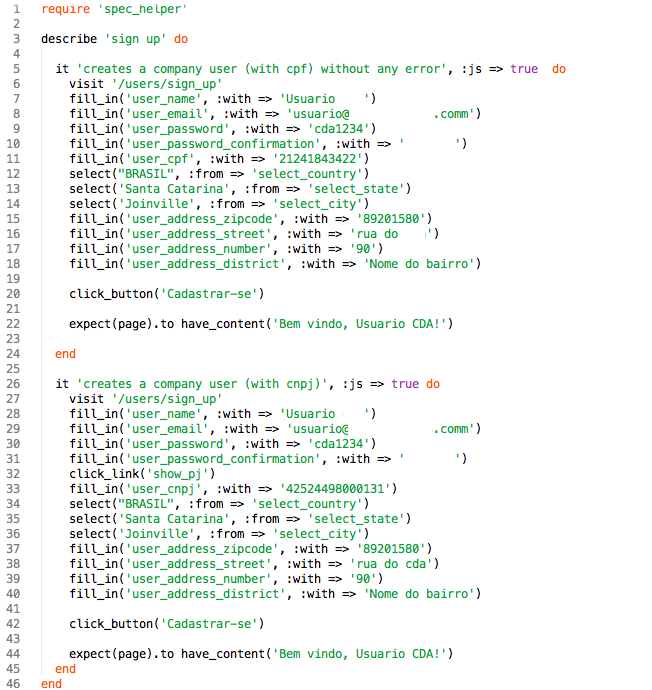
\includegraphics[width=15cm]{assets/teste_view} \\
\fonte{Autoria própria.}
\end{center}
\end{figure}

A Figura \ref{fig:teste_view} mostra um teste de \textit{view} para o cadastro. Basicamente ele testa a criação de um usuário normal sem erro algum e a criação de um usuário do tipo pessoa jurídica sem erro algum. Como o sistema trata da criação de autores também, que podem ser pessoa física ou jurídica, os testes para esses casos também devem ser implementados. Ao final deve haver os seguintes testes: pessoa física não autora, pessoa física autora, pessoa jurídica não autora e pessoa jurídica autora.

Ao rodar os testes, o \textit{browser} abrirá e os dois casos são testados. Caso o comportamente no bloco expect não aconteça, o teste falhará.

Esse tipo de abordagem e teste demonstra ser interessante em sistemas legados e com poucos teste, pois futuramente não precisa se gastar tempo testando manualmente se uma dada funcionalidade do sistema está funcionando ou não. Esse código ainda pode ser melhorado para eliminar duplicidade (conforme o \textit{seiso} ou limpeza do 5S). Muitos campos estão sendo testados com o mesmo nome, logo eles poderiam estar numa função que é chamada antes de entrar em cada bloco it.

Outra forma de incorporar qualidade no serviço é utiliza-se de ferramentas de métricas que avaliam a complexidade do código e ferramentas que analisam os erros que ocorrem em ambiente de produção. Uma ferramenta desse tipo pode ser o Airbrake, que é mostrada na Figura \ref{fig:airbrake}. Caso aconteça algum erro em algum ambiente, a empresa é notificada e pode tomar alguma ação antes de receber uma reclamação ou que alguma coisa mais séria aconteça. Programas que avaliam métrica do sistema como complexidade cicliomática, podem indicar locais do código com alta complexidade, e que possivelmente são mais difíceis de serem mantidos ou que possuem algum erro.

\begin{figure}[htb!]
\begin{center}
\caption{Ferramenta de detecção de bugs}
\label{fig:airbrake}
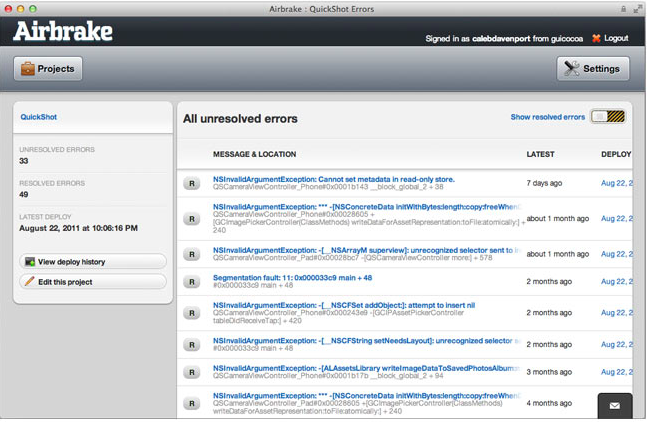
\includegraphics[width=15cm]{assets/airbrake} \\
\fonte{Autoria própria.}
\end{center}
\end{figure}

\section{ORGANIZANDO O TRABALHO}

Um componente muito utilizado pelas empresas, e que foi implantado de modo eletrônico, vindo do \textit{lean} foi o Kanban. Segundo \citeonline{poppendieck:10}, a palavra kanban significa cartão e é utilizada na manufatura para indicar o trabalho que precisa ser feito. O kanban pode ser utilizado no desenvolvimento de \textit{software} para indicar o andamento de uma funcionalidade no fluxo de produção. Para o \textit{kanban}, há uma coluna para cada passo dentro do fluxo de trabalho da empresa. Tudo isso pode ser feito em nível mais abrangente, como as histórias de usuário, como mais técnicos como as implementações necessárias para uma funcionalidade.

Os sistemas de \textit{kanban} são projetados para limitar o trabalho que está sendo executado, pois quanto mais processos estão sendo executados, mais lento é o fluxo de trabalho. Essa é a principal razão da invenção do \textit{kanban}, segundo \citeonline{poppendieck:10}, ou seja limitar o trabalho que está sendo executado e melhorar o fluxo no processo. A Figura \ref{fig:kanban} mostra um exemplo de um quadro. Cada coluna representa um passo, ou etapa no fluxo de trabalho de uma empresa. No exemplo da figura cada funcionalidade chega ao quadro pelo lado esquerdo na coluna ``\textit{Next Features}''. O número máximo de funcionalidades que devem ficar nessa coluna são três. Quando há  espaço suficiente, a funcionalidade muda de estado. No próxima etapa, a funcionalidade é decomposta em histórias e depois são postas na próxima coluna. O fluxo segue através do desenvolvimento e testes unitários e depois para o teste de aceitação. Uma vez que uma funcionalidade passe no teste de aceitação, elas são transformadas em funcionalidades novamente e passam pelo teste de aceitação de funcionalidade e \textit{staging}. Finalmente, a funcionalidade é colocado na coluna de pronto (\textit{Ready to Release}).

O membro do time pode trabalhar em qualquer etapa que tiver habilidade. Quando uma funcionalidade termina, o tempo para que ela se movesse através do quadro de \textit{kanban} é anotado. O dia em que a funcionalidade foi posta em ``\textit{Next Features}'' é subtraído do dia em que ela entrou em ``\textit{Ready to Release}''. O resultado é então colocado no gráfico ``\textit{Days to Complete Feature}'' (dias para completar a funcionalidade).

\begin{figure}[htb!]
\begin{center}
\caption{Exemplo de um kabban}
\label{fig:kanban}
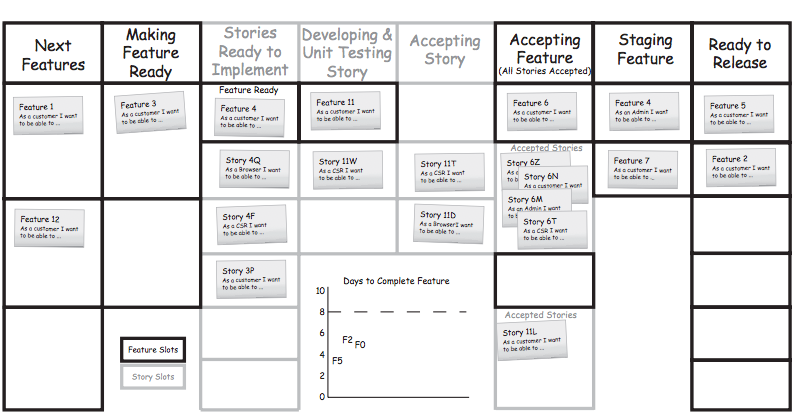
\includegraphics[width=14cm]{assets/kanban} \\
\fonte{\citeauthoronline{poppendieck:10}, \citeyear{poppendieck:10}.}
\end{center}
\end{figure}

Existem outras variações do \textit{kanban} e na empresa foi implementada uma versão eletrônica utilizando-se da ferramenta Trello\footnote{O trello é uma ferramenta livre e pode ser utilizado através do endereço http://bit.ly/1eyOBPE}. Na empresa, foi utilizado os seguintes passos (para uma funcionalidade), To--Do, Em Execução, Feito e parado. Algumas informações forem omitidas na imagem para preservar a empresa. O exemplo do \textit{kanban} pode ser visto na Figura \ref{fig:trello}.

\begin{figure}[htb!]
\begin{center}
\caption{Exemplo de kabban na empresa}
\label{fig:trello}
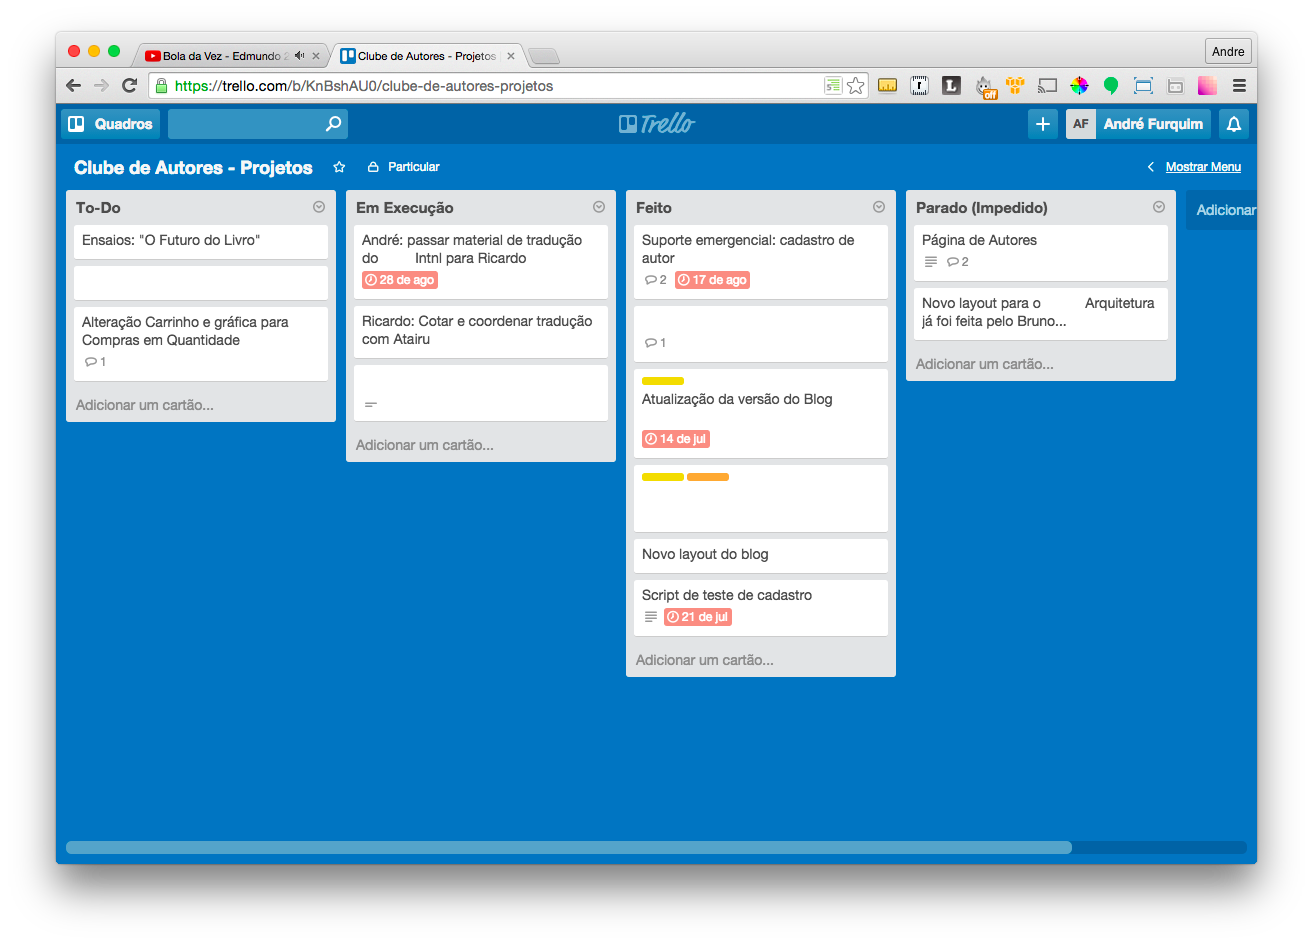
\includegraphics[width=14cm]{assets/trello} \\
\fonte{Autoria própria.}
\end{center}
\end{figure}

\section{CONCLUSÃO DO CAPÍTULO}

Nesse capítulo foram vistos alguns problemas da empresa e suas soluções aplicando os princípios \textit{lean} de desenvolvimento de \textit{software}. Foi visto que algumas demandas de suporte foram diminuidas através da utilização de teste não apenas depois da implementação de uma funcionalidade, para ver se tudo funciona conforme o desenvolvimento, mas de maneira preventiva ou trabalhando-se na sua detecção. Para melhorar o processo da empresa é fundamental que seja entendido o seu fluxo e que seus desperdícios sejam eliminados. Existe várias outras técnicas, em nível de programação, que também pode auxiliar no processo e que acabaram sendo incorporadas e que foram identificadas na sessão \ref{lean:org}. No próximo capítulo é feita a conclusão sobre o trabalho realizado.